% % % % % % % % % % % % % % % % % % % % % % % % % % % % % % % % % % % % % % % % % % % %
%                                                                                     %
% Short Sectioned Assignment LaTeX Template Version 1.0 (5/5/12)                      %
% This template has been downloaded from: http://www.LaTeXTemplates.com               %
%                                                                                     %
% Original author:  Frits Wenneker (http://www.howtotex.com)                          %
%                                                                                     %
% Modified by: Fco Javier Sueza Rodríguez (fcosueza@disroot.org)                      %
%                                                                                     %
% Changes:                                                                            %
%	    - Custom Chapters, Sections and Subsections (titlesec package)                %
%           - Document type scrbook (oneside)                                         %
%           - Use babel-lang-spanish package and marvosym                             %
%           - Use hyperref, enumitem, tcolorbox and glossaries packages               %
%           - Use Time New Roman (mathptmx), Helvetic and Courier fonts               %
%                                                                                     %
% License: CC BY-NC-SA 3.0 (http://creativecommons.org/licenses/by-nc-sa/3.0/)        %
%                                                                                     %
% % % % % % % % % % % % % % % % % % % % % % % % % % % % % % % % % % % % % % % % % % % %

%-----------------------------------------------%
%	              Packages                  %
%-----------------------------------------------%

\documentclass[paper=a4, fontsize=11pt, oneside]{scrbook}

% ---- Text Input/Output ----- %

\usepackage[T1]{fontenc}
\usepackage[utf8]{inputenc}
\usepackage{mathptmx}
\usepackage[scaled=.92]{helvet}
\usepackage{courier}
\usepackage[indent=12pt]{parskip}

\usepackage{geometry}
\geometry{verbose,tmargin=3cm,bmargin=3cm,lmargin=2.6cm,rmargin=2.6cm}

% ---- Language ----- %

\usepackage[spanish]{babel}
\usepackage{marvosym}

% ---- Another packages ---- %

\usepackage{amsmath,amsfonts,amsthm}
\usepackage{graphics,graphicx}
\usepackage{titlesec}
\usepackage{fancyhdr}
\usepackage{tcolorbox}
\usepackage{hyperref}
\usepackage{enumitem}
\usepackage[automake]{glossaries}

%--------------------------------------------------------------------%
%                      Customizing Document                          %
%--------------------------------------------------------------------%


% ----------- Custom Chapters, Sections and Subsections -------------- %

\titleformat{\chapter}[display]
			{\bfseries\Huge}
			{Tema \ \thechapter} {0.5ex}
			{\vspace{1ex}\centering}

\titleformat{\section}[hang]
			{\bfseries\Large}
			{\thesection}{0.5em}{}

\titleformat{\subsection}[hang]
			{\bfseries\large}
			{\thesubsection}{0.5em}{}

\titleformat{\subsubsection}[hang]
			{\bfseries\large}
			{\thesubsubsection}{0.5em}{}

\hypersetup{
    colorlinks=true,
    linkcolor=black,
    urlcolor=magenta
}

% ------------------- Custom heaaders and footers ------------------- %

\pagestyle{fancyplain}

\fancyhead[]{}
\fancyfoot[L]{}
\fancyfoot[C]{}
\fancyfoot[R]{\thepage}

\renewcommand{\headrulewidth}{0pt} % Remove header underlines
\renewcommand{\footrulewidth}{0pt} % Remove footer underlines

\setlength{\headheight}{13.6pt} % Customize the height of the header

% --------- Numbering equations, figures and tables ----------------- %

\numberwithin{equation}{section} % Number equations within sections
\numberwithin{figure}{section} % Number figures within sections
\numberwithin{table}{section} % Number tables within sections

% ------------------------ New Commands ----------------------------- %

\newcommand{\horrule}[1]{\rule{\linewidth}{#1}} % Create horizontal rule command


%----------------------------------------------------------------------------------------
%	TÍTULO Y DATOS DEL ALUMNO
%----------------------------------------------------------------------------------------

\title{
\normalfont \normalsize
\textsc{{\bfseries Curso 2022-2023} \\ Ciclo Superior de Desarrollo de Aplicaciones Web \\ IES Aguadulce} \\ [25pt]
\horrule{0.5pt} \\[0.4cm]
\huge Sistemas Informáticos \\
\horrule{0.5pt} \\[0.4cm]
}

\author{Francisco Javier Sueza Rodríguez}
\date{\normalsize\today}

%----------------------------------------------------------------------------------------
%                                     DOCUMENTO
%----------------------------------------------------------------------------------------
\makeglossaries
\loadglsentries{glossary.tex}

\begin{document}

\maketitle

\newpage

\tableofcontents

\listoffigures

%\listoftables

\newpage

\chapter{Hardware de un Sistemas Informático}
En esta primera unidad de la asignatura ``\textbf{Sistemas Informáticos}, vamos a ver los conceptos básicos de sobre los sistemas informáticos, centrándonos principalmente en el apartado del hardware de un sistema informático. Así, veremos cuales son los diferentes componente hardware (o físicos) de un computador, así como la información necesaria para su ensamblaje y puesta en marcha.

También veremos diferentes tipos de clasificaciones de los ordenadores, incluyendo los ordenadores personales, así como otra información útil que podremos encontrar en los diferentes anexos que se incluyen al final de esta unidad.

\section{Sistema Informático}
La \textbf{informática} es la ciencia que se encarga de estudiar todo lo relacionado con los sistemas informáticos, incluyendo los temas relativos a su arquitectura y fabricación, hasta los temas referidos al almacenamiento y organización de la información, sin olvidar la creación y uso de software, o la formación del personal informático. Para ello, se apoya en múltiples disciplinas como las matemáticas, física, electrónica, etc...

Un \textbf{sistema informático} es el conjunto de \textbf{elementos físicos} (hardware) y \textbf{elementos lógicos} (software), interconectados entre sí, destinados a gestionar el \textbf{tratamiento automático de la información}, entendiendo por esto, su almacenamiento, transmisión, organización y/o procesamiento.

Se incluye, como parte fundamental de un sistema informático, al \textbf{conjunto de personas} que lo \textbf{utiliza}, ya sean usuario, administradores, programadores, etc... El elemento humano es un \textbf{componente imprescindible}, ya que los sistemas informáticos son creados, desarrollados y utilizados por humanos para su propio provecho.

En sistema informáticos siempre debemos distinguir entre hardware y software:

\begin{itemize}
    \item \textbf{Hardware}: son todos los elementos físicos que forman parte de un ordenador, es decir, teclado, ratón, placa base, monitor, memoria, disco duro, cables, etc... Es la ``maquinaria'' necesaria utilizada para el tratamiento de la información.
    \item \textbf{Software}: es el elemento lógico e ``intangible'' de un sistema informático. Se compone de un conjunto de programas y datos que permiten manejar el hardware, controlando y coordinando su funcionamiento para que pueda realizar las tareas esperadas. Esta compuesto principalmente de dos elementos:
    \begin{itemize}
        \item \textbf{Programas}: están formados por un conjunto de órdenes o instrucciones que se utilizan para procesador los datos que se introducen como información. Son necesarios para la gestión y el control de los equipos y los trabajos de los usuarios.
        \item \textbf{Datos}: son la información que los programas deben procesar, utilizando para esto diferentes elementos hardware que componen el sistema informático. Son, en definitiva, la razón de ser el sistema informático.
    \end{itemize}
\end{itemize}

Los \textbf{sistemas informáticos} han \textbf{evolucionado}. En un principio todos sus componentes, físicos, lógicos y humanos, estaban localizados en el mismo lugar, pero actualmente están formados por subsistemas que se interconectan a través de la red, que pueden llegar a estar a miles de kilómetros de distancia entre sí, integrando sistemas complejos de procesamiento de la información. Estos subsistemas a si vez pueden estar compuestos por un superodenador, un ordenador personal, redes locales de ordenadores o por una combinación de todos ellos, siendo el sistema informático más simple el formado por un ordenador y un usuario que ejecuta programas en él.

Un \textbf{ordenador} se define como una máquina electrónica, con algunas partes mecánicas, compuesta por al menos, una unidad de proceso, y por equipos periféricos, controlada por programas que deben estar almacenados en su memoria central, destinada al tratamiento automático de la información que le es suministrada. Es una máquina de propósito general ya que puede realizar gran variedad de trabajos y a gran velocidad.

En el \textit{Anexo A.1}, podrás encontrar más información sobre la clasificación de los ordenadores.

\section{Arquitectura Hardware: Componentes Funcionales}
Un computador esta compuesto por una seria de sistemas y subsistemas hardware, que cooperando entre sí, permiten a este llevar a cabo su función, procesando la información que recibe y emitiendo los resultados de este procesado.  En la siguiente figura vemos un esquema de estos subsistemas.

\begin{figure}[ht]
    \centering
    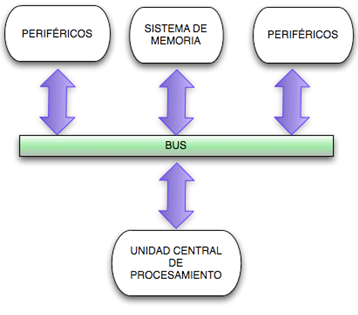
\includegraphics[scale=0.90]{arquitectura-computador.png}
    \caption{Subsistemas de la arquitectura de un computador}
\end{figure}


Como vemos en la imagen, hay tres subsistemas principales, que son los siguientes:

\begin{itemize}
    \item \textbf{Unidad Central de Proceso} (CPU): es el sistemas básico más importante, encargado de coordinar a los demás subsistemas, extraer secuencialmente las instrucciones de la memoria principal para procesarlas y ejecutarlas.
    \item \textbf{Sistemas de Memoria}: su función básica es la de almacenar las instrucciones que se van a procesar posteriormente, los datos y los resultados que sean necesarios.
    \item \textbf{Periféricos}: se dividen en periféricos de entrada y de salida, según la dirección del flujo de información. Ambos sistemas se encargan de la comunicación con el exterior, es decir, con el usuario u otros sistemas.
\end{itemize}

Además de estos tres subsistemas, debemos de hablar de \textbf{bus de sistema}, que es el medio físico encargado de transmitir la información entre los diferentes subsistemas.

En la actualidad, la arquitectura empleada es la fabricación de computadores es la \textbf{arquitectura Von Neumann}. Esta arquitectura de computadoras ésta basada en la descrita en 1945 por el matemático y físico \textbf{John Von Neumann}. En la siguiente imagen podemos ver un esquema de la arquitectura Von Neumann.

\begin{figure}[ht]
    \centering
    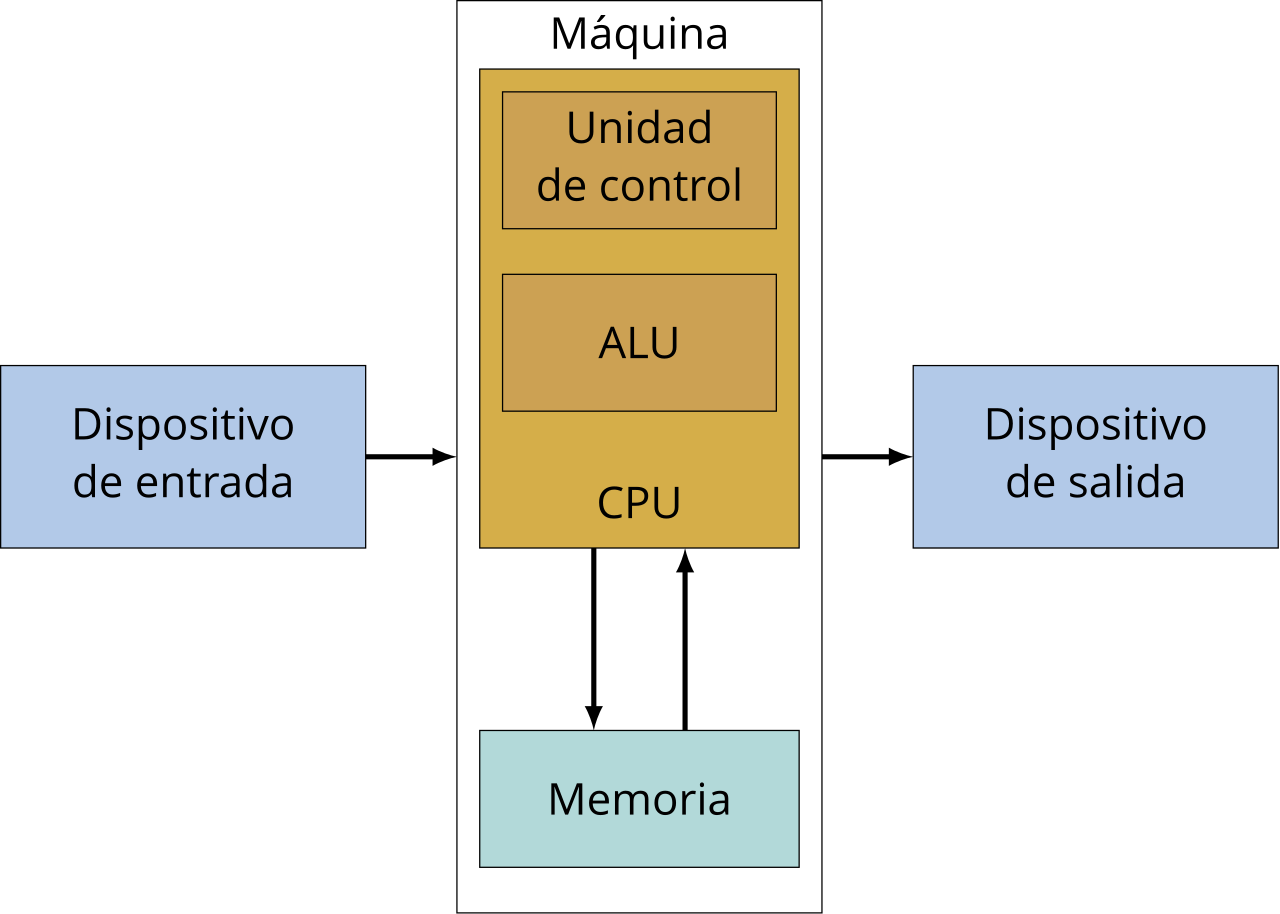
\includegraphics[scale=0.25]{von-neumann.png}
    \caption{Arquitectura Von Neumann}
\end{figure}

Como vemos es igual a la que hemos descrito en este punto. Podemos observar como la \textbf{CPU} contiene dos unidades, la \textbf{unidad de control} y la \textbf{ALU} o \textbf{unidad Aritmético-Lógica}, las cuales veremos con más detalle en la siguiente sección.

Si queremos saber más sobre esta arquitectura, lo cual recomiendo encarecidamente, podemos visitar \href{https://es.wikipedia.org/wiki/Arquitectura_de_Von_Neumann}{la entrada en Wikipedia} de la arquitectura Von Neumann.

\subsection{Componentes Principales (CPU, RAM, E/S, ...)}
La \textbf{Unidad Central de Proceso} es el componente que podría definirse como el ``cerebro'' del computador, ya que es la encargada de controlar, dirigir y coordinar todas las operaciones que realiza el ordenador.

Para que la CPU pueda ejecutar un \textbf{\gls{programa}} es necesario que éste se guarde en su memoria principal, desde donde se van extrayendo en secuencia cada una de sus instrucciones, analizándolas y emitiendo las órdenes necesarias al resto de componentes que deban intervenir para completar su ejecución.

La CPU esta integrada en el Procesador Central o microprocesador y acompañada de una pequeña cantidad de \textbf{\gls{registros}} de memoria necesarios para su funcionamiento.

Dentro del Microprocesador, y como parte integrante de la \textbf{CPU}, existen dos unidades, como ya vimos en el apartado anterior sobre la arquitectura Von Neumann. Esta unidades son:

\begin{itemize}
    \item \textbf{Unidad de Control}: se encarga de ejecutar los programas, controlando su secuencia, interpretando y ejecutando las instrucciones. Se encarga también de controlar al resto de componentes, como periféricos, memoria, etc.., según vayan necesitando las instrucciones.
    \item \textbf{Unidad Aritmético-Lógica} o \textbf{ALU}: se encarga de realiza los cálculos matemáticos y lógicos necesarios para su funcionamiento.
\end{itemize}

La memoria principal, conocida como \textbf{RAM} (Random Access Memory), es la encargada de almacenar los datos e instrucciones de los programas que deben ejecutarse, así como toda la información que el sistema necesita para su funcionamiento. Esta constituida por un \textbf{conjunto de registros} capaces de retener información en su interior mientras el ordenador esta en funcionamiento. Cuando el ordenador se apaga, se pierde su contenido, por lo que esta memoria es de tipo \textbf{\gls{volatil}}.

Los \textbf{sistemas de Entrada y Salida} son circuitos electrónicos que permiten el intercambio de información entre la CPU y los periféricos. Las unidades de entrada y salida se usan para cargar programas y datos en memoria principal desde los periféricos de entrada, y las unidades de salida para mostrar los resultados de las operaciones realizadas a través de periféricos de salida.

Los \textbf{buses del sistema} son el conjunto de circuitos eléctricos que conectan la CPU con el resto de componentes para comunicarse entre sí. Cada bus es un conjunto de cables de un circuito integrado que permite la transmisión de información de forma paralela. Podemos encontrar tres tipos diferentes de buses:

\begin{itemize}
    \item \textbf{Bus de Instrucciones y Datos}: se utilizan para trasladar tanto instrucciones como datos desde la memoria RAM al resto de componentes del computador y viceversa.
    \item \textbf{Bus de Control}: bus que se encarga de trasmitir las instrucciones desde la CPU al resto de unidades y recibe de ellas señales indicando su estado.
    \item \textbf{Bus de Direcciones}: se encarga de transmitir las direcciones de destino de los datos que se envían por el bus de datos.
\end{itemize}

En la siguiente figura, podemos ver un esquema con todos estos componentes.

\begin{figure}[ht]
    \centering
    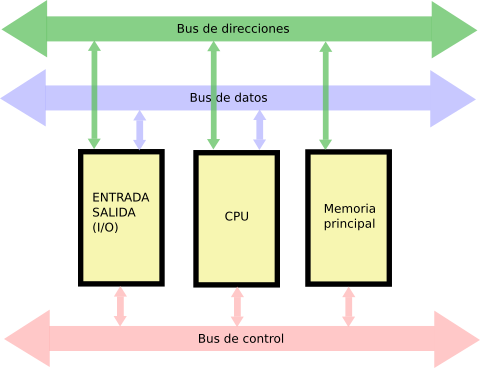
\includegraphics[scale=0.46]{buses-de-sistema.png}
    \caption{Unidades y buses del sistema}
\end{figure}

\subsection{Periféricos y Almacenamiento Externo}
Los \textbf{periféricos} son los dispositivos electrónicos, unidades externas, que se conectan al ordenador a través de los buses de entrada/salida, integrándose en el sistema, que pasa a controlarlos como parte de sí mismo desde el momento en el que se reconoce su conexión.

Existen infinidad de periféricos, diferentes por su diseño y función. Algunos tienen como finalidad facilitar la entrada de información en el ordenador, mientras que otros facilitan su salida, otros cuya finalidad es el almacenamiento permanente de datos o los que permiten la conexión con otras máquinas y el intercambio de información. No todos ellos son imprescindibles, aunque los más normal es contar de teclado, ratón, monitor, impresora altavoces y conexión de red.

Los periféricos se pueden clasificar, según su función, en los siguientes:

\begin{itemize}
    \item \textbf{Unidades de Entrada}: son aquellos periféricos que permiten introducir la información o los datos desde el exterior a la memoria principal, preparando la información para que pueda ser procesada por la máquina. Un ejemplo de estos periféricos son el teclado y el ratón.
    \item \textbf{Unidades de Salida}: son las encargadas de sacar al exterior los datos resultantes de las operaciones realizadas, mostrando la información de forma comprensible para el usuario. Ejemplos de estas unidades son la pantalla o la impresora.
    \item \textbf{Unidades de Entrada/Salida}: esta unidades de usan tanto para entrada como para la salida de información del sistema. Algunas de estas unidades no necesitan hacer procesos de conversión ya que manejan la información en formato binario, mientras que otras necesitan procesos de conversión para trabajar con los usuarios o para comunicarse con otro dispositivo. Algunos ejemplos son las tarjetas de red, discos duros, memorias USB, etc...
\end{itemize}

Algunos periféricos necesitan \textbf{soportes adicionales} para representar la información o almacenarla. En estos casos hay que tener en cuenta que el periférico no almacena la información, sino que es el medio utilizado para obtener o almacenar la información en su soporte. Un ejemplo de esto son los lectores de DVD o Blu-Ray.

\section{Componentes Físicos de un Ordenador Actual}
La arquitectura de un ordenador define la estructura funcional de cada una de sus partes, pero se hace necesario implementar dicha estructura mediante hardware de fabricación y comercialización actual. Dependiendo de  las características tecnológicas de los componentes empleados en su construcción (tamaño, grado de miniaturización, capacidad de procesado, ...), se ensamblarán ordenadores personales más o menos potentes, como portátiles, tablets, smartphones, consolas de juegos, etc... Pero también servidores, mainframes y superordenadores.

Hay que tener en cuenta, que los distintos componentes deben seguir unos estándares de fabricación, especialmente en lo relativo a sus conexiones y \textbf{\gls{interfaces}}, para permitir su completa integración con el sistema y mantener la compatibilidad de funcionamiento entre ellos.

En esta sección vamos a hacer un estudios de los diferentes elementos utilizados para el ensamblaje de un ordenador personal de sobremesa de uso general en base a componentes físicos que se fabrican y comercializan en la actualidad. Analizando en la medida de lo posible sus características de funcionamiento particulares.

\subsection{Cajas de Ordenador}
La \textbf{caja del ordenador}, también conocida como carcasa o chasis, es el ``recipiente'' donde se colocan todos los componentes del ordenador y que sirve para protegerlos. Estas cajas se fabrican en diversos materiales como acero, aluminio, plástico, metacrilato, etc.., o con una combinación de estos. Deben tener la suficiente resistencia para soportar el peso de los componentes en su interior, así como el calor que estos generan y suficiente espacio para albergarlos a todos con una distribución adecuada.

Estás cajas se fabrican siguiendo unos diseños de basados en unos \textbf{factores de forma} estándares, cada uno con sus propias características de tamaño, forma, capacidad, etc. Los principales factores de forma que nos podemos encontrar son los siguientes:

\begin{itemize}
    \item \textbf{Minitorre o Semitorre}: la diferencia entre ellas está en la altura y el número de \textbf{\gls{bahias}} de 5 y cuarto de que dispongan. A mayor número de bahías, más dispositivos podrá contener y más aumenta su altura. Suelen tener entre 2 y 4 bahías respectivamente.
    \item \textbf{Sobremesa}: son similares a las semitorres pero se colocan de forma horizontal, lo que obliga a rotar 90 grados los dispositivos extraíbles de su frontal.
    \item \textbf{Barebone y Slim}: son cajas de pequeño tamaño principalmente diseñadas para ocupar poco espacio. Esto implica que su interior admite pocos dispositivos, o ninguno, pero se compensa aumenta el número de conectores para dispositivos externos.
\end{itemize}


% Glossary

\glsaddall
\printglossaries

% Bibliography

\newpage
\addcontentsline{toc}{chapter}{Bibliografía}
\bibliography{citas}
\bibliographystyle{unsrt}

\end{document}